\namedsection{Domänenmodelle}{J}
Domänenmodelle bilden die benötigte Struktur der Daten für einen festgelegten Anwendungszweck ab. Im Falle von Statistance sollen Daten für spätere statistische Analysen aus Drittsystemen bezogen werden. Dementsprechend müssen all jene Datenfelder abgedeckt werden die für die statistische Auswertung von Statistance unabdingbar sind.

Zudem sollte das Domänenmodell möglichst allgemein gehalten werden um den Aufwand für das Hinzufügen von weiteren Drittsystemen zu reduzieren, siehe auch den Abschnitt \ref{sec:non-functional} Anpassbarkeit. Andernfalls verhindert es eine Lösung die möglichst skalierbar ist, weil es wiederholt zu einem Änderungsbedarf des Modells führen kann.
\begin{figure}[!h]
\centering
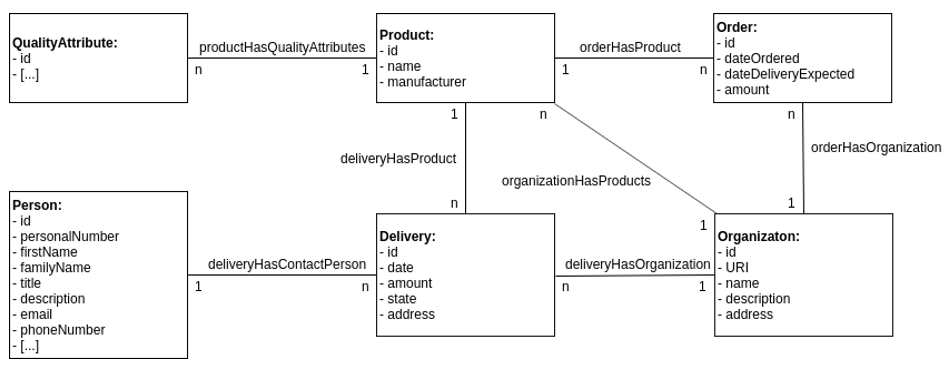
\includegraphics[width=15cm]{images/0x_requirement_analysis/potential_domainmodels.png}
\caption{Mögliches Domänenmodell Diagramm aus vorläufigen Vorgaben}
\label{fig:preliminary_domain_model}
\end{figure}

Im Diagram der Abbildung \ref{fig:preliminary_domain_model} lässt sich bereits ein Modellierung erkennen die aus den zwischenzeitlichen Vorgaben von Statistance entstanden ist. Letztendlich deckte sich diese Modellierung aber nicht mit den vorhanden Daten aus dem Drittsystemen. Deshalb hat es am Ende nochmal eine größere Veränderung durchgemacht.

Organization wurde aufgeteilt in Lieferant und Hersteller. Eine Bestellung und Lieferung erhält nun zusätzliche Informationen über die beinhalteten Produkte. Viele Felder konnten nicht über die vorhandenen Daten abgedeckt werden und sind daher ausgelassen. Darüber hinaus gibt es auch keinerlei Informationen über Qualitätsattribute aber Produkte wurden zumindest um Kategorien unterschiedlicher Ebenen ergänzt.

\namedsection{Datenmapping}{J}
Beim Mapping der Daten ist die Vollständigkeit auch immer von der Pflege der Daten abhängig. Ebenso hat es einen Einfluss wie genau sich der Nutzer eines ERP-Systems an bestehende Konventionen des Systems hält. Weil dies nicht immer gegeben ist, und ERP-Systeme stark angepasst werden können, kann es passieren, dass die benötigte Daten bei gleicher Version eines ERP-System bei unterschiedlichen Kunden, in abweichende Tabellen abegelegt sind. Demzufolge kann das korrekte Mapping für neue Kunden mit ähnlichen Vorbedingungen nicht grundsätzlich gewährleistet werden. Zum Beispiel haben sich bereits die Lage der Daten zwischen Testinstanz und Pilotkunden teilweise stark unterschieden.

Deshalb geht es speziell in diesem Abschnitt um das Mapping der Daten aus dem Sage 100 Drittsystem eines Pilotkundens. Dazu werden für jede erforderte Entität die benutzte SQL-Abfrage dargelegt und beschrieben wie sich die Daten schlussendlich zusammensetzen.

\subsection{Produkte}
Produkte aus Sage 100 können entweder gelieferte Komponenten für eigene Kreationen sein oder die vom Unternehmen verkauften Produkte.

In Falle von Statistance interessieren uns vor allem Artikel die von Lieferanten gebracht werden. Vornehmlich besteht ein Produkt aus der Artikelnummer, einer menschenfreundlichen Bezeichnung und unterschiedlichen Artikelgruppen. Speziell die Kategorien können wohlmöglich in statistischen Analysen verwendet werden, weil Qualitätskriterien propagieren.
\begin{lstlisting}[language=SQL,caption=Artikel Join SQL Query]
SELECT
   A.Artikelnummer, CONCAT(A.Bezeichnung1, A.Bezeichnung2) as Bezeichnung,
   A.Hersteller, A.Timestamp, A.Artikelgruppe, A.Vaterartikelgruppe,
   A.Hauptartikelgruppe,
   AG1.Bezeichnung as Hauptartikelgruppebezeichnung,
   AG2.Bezeichnung as Vaterartikelgruppebezeichnung,
   AG3.Bezeichnung as Artikelgruppebezeichnung
FROM KHKArtikel as A
LEFT OUTER JOIN KHKArtikelgruppen AG1
    ON AG1.Hauptartikelgruppe = A.Hauptartikelgruppe
    AND AG1.Gruppenebene = 1
LEFT OUTER JOIN KHKArtikelgruppen AG2
    ON AG2.VaterArtikelgruppe = A.Vaterartikelgruppe
    AND AG2.Gruppenebene = 2
LEFT OUTER JOIN KHKArtikelgruppen AG3
    ON AG3.Artikelgruppe = A.Artikelgruppe
    AND AG3.Gruppenebene = 3
\end{lstlisting}

\subsection{Lieferanten}
In der Domäne von Statistance liefert diese Entität die Artikel aus der Produkt-Entität an das Unternehmen aus. Neben der Lieferadresse enthält es Informationen über Ansprechpartner.
\begin{lstlisting}[language=SQL,caption=Zulieferer Join SQL Query]
SELECT
    A.Matchcode as id, A.Homepage as uri, A.Adresse as adresseId,
    CONCAT(A.Name1, A.Name2) as name, A.LieferStrasse, A.LieferPLZ,
    A.LieferLand, A.LieferOrt, A.LieferZusatz,
    AP.Nummer, AP.Ansprechpartner, AP.Abteilung, AP.Telefon,
    AP.Telefax, AP.EMail, AP.Mobilfunk
FROM KHKAdressen as A
LEFT OUTER JOIN KHKAnsprechpartner AP
    ON A.Adresse = AP.Adresse
WHERE A.Gruppe = 'LIEF'
\end{lstlisting}

\subsection{Bestellungen}
Bevor Produkte geliefert werden findet eine Bestellung statt. Bestellungen sind eng mit den Tabellen für Belege aus dem Sage 100 System verbunden. Relevant sind hierbei das Belegdatum, Liefertermin sowie Informationen über die Einzelposten der Bestellung mitsamt der Angaben der Menge, Artikelnummer und Adresse.
\begin{lstlisting}[language=SQL,caption=Bestellungen Join SQL Query]
SELECT
    B.BelID as belId, B.Belegnummer as belegnummer, B.Belegdatum as belegdatum,
    B.Liefertermin as lieferdatum, B.A0MatchCode as a0MatchCode,
    BP.BelPosID as belPosId, BP.Artikelnummer as artikelnummer, BP.Bestellnummer,
    BP.Liefertermin as positionLiefertermin, BP.Menge as menge,
    BP.Mengeneinheit as mengeneinheit, CONCAT(BP.Bezeichnung1, BP.Bezeichnung2) as bezeichnung,
    A.Homepage as uri, A.Adresse as adresseId, CONCAT(A.Name1, A.Name2) as adresseName,
    A.LieferStrasse as adresseStrasse, A.LieferPLZ as adressePlz, A.LieferOrt as adresseOrt,
    A.LieferLand as adresseLand, A.LieferZusatz as adresseZusatz
FROM KHKEKBelege as B
         left outer join KHKEKBelegePositionen BP on B.BelID = BP.BelID
         left outer join KHKAdressen A on B.A0MatchCode = A.MatchCode
WHERE B.Belegart = 'Bestellung'
\end{lstlisting}

\subsection{Lieferungen}
Lieferungen haben stattgefunden sobald eine Bestellung im Lager eintrifft. Lieferungen sind ebenfalls eng mit den Tabellen für Belege aus dem Sage 100 System verbunden. Auch hier wieder relevant sind das Belegdatum, Liefertermin sowie Informationen über die Bestandteile der Lieferung mitsamt der Angaben über die Menge, Artikelnummer und Adresse.
\begin{lstlisting}[language=SQL,caption=Lieferungen Join SQL Query]
SELECT
    B.BelID as belId, B.Belegnummer as belegnummer,
    B.Belegdatum as belegdatum, B.Liefertermin as lieferdatum,
    B.A0MatchCode as a0MatchCode, B.Lieferschein, B.ReferenzBelID,
    BP.BelPosID as belPosId, BP.Artikelnummer as artikelnummer,
    BP.Liefertermin as positionLiefertermin, BP.Menge as menge,
    BP.Mengeneinheit as mengeneinheit, CONCAT(BP.Bezeichnung1, BP.Bezeichnung2) as bezeichnung,
    A.Homepage as uri, A.Adresse as adresseId, CONCAT(A.Name1, A.Name2) as adresseName,
    A.LieferStrasse as adresseStrasse, A.LieferPLZ as adressePlz, A.LieferOrt as adresseOrt,
    A.LieferLand as adresseLand, A.LieferZusatz as adresseZusatz
FROM KHKEKBelege as B
    left outer join KHKEKBelegePositionen BP on B.BelID = BP.BelID
    left outer join KHKAdressen A on B.A0MatchCode = A.MatchCode
WHERE B.Belegart = 'Wareneingang'
\end{lstlisting}

\subsection{Mitarbeiter}
Speziell bei dieser Entität gab es die größten Unterschiede zwischen Testinstanz und dem Snapshot des Pilotkunden. Mitarbeiterdaten wurden nicht in die Tabelle für Adressen gepflegt. Deshalb gibt es vorwiegend nur Informationen über die Namen der Mitarbeiter.
\begin{lstlisting}[language=SQL,caption=Mitarbeiter SQL Query]
SELECT CONCAT(Nummer, Mandant) as id, Matchcode as name FROM KHKMitarbeiter
\end{lstlisting}

\subsection{Hersteller}
Angaben über die Hersteller lassen sich normalerweise über die Spalte Hersteller aus der Artikel-Tabelle entnehmen. Jedoch wie im Falle der Mitarbeiter wurden diesen Daten nicht eingepflegt, weswegen nahezu keine Informationen für diese Entität vorliegt. In vier Fällen (von zehntausenden) liegt eine Herstellerangabe vor aber ohne weitere Verknüpfung in anderen Tabellen.